\documentclass{article}
\usepackage{graphicx}
\usepackage{hyperref}
\usepackage{amsmath} 

\title{Franka Research 3 Bimanual}
\author{Alessandro Moscatelli}
\date{July 2025}

\begin{document}

\maketitle

\section{Introduction}

This report serves as documentation for setting up a bimanual workspace for two Franka Research 3 robots. In the first place it is described how the custom-defined hardware interface works and it's sub-modules. Then, some simple controller approach and utilities of the Franka Multi Manual Package are described, continuing with the definition of the URDF and the launch file for the two robots. The report is concluded with a small talk on how to set up a different DDS and some possible troubleshooting.

\section{Requirements}
This small section serves as a list of the requirements to correctly run this project:
\begin{itemize}
    \item Linux Real-Time Kernel
    \item ROS2 Humble
    \item Libfranka 0.15.0
    \item Franka Description, version 1.0.2
    \item Franka ROS2 control library, version 2.0.1
\end{itemize}

\section{Franka multi-manual hardware interface}
This is the core package of this project that implements a ROS2 Hardware Interface for precise concurrent control of a maximum of N robots. This custom definition of the interface is done to have a no-delay precision when controlling the robot simultaneously, an unachievable objective using two independent hardware interfaces. This package is divided into sub-modules, which are given a high-level description, fully documented at this \href{https://idra-lab.github.io/idra-franka-launch/#doxygen}{link}. 

\textbf{franka\_mm\_hardware\_interface} is the class that implements the logic of the hardware interface used by ROS2, extending the class \texttt{SystemInterface} and thus inheriting all its methods. The core tasks done by this class are: 
\begin{itemize}
    \item Instantiate the robot objects used to maintain the connection between the interface and the real robot.
    \item Export state and command interfaces, used to read and write state and desired commands on the robot.
    \item Handle controller switches and instantiation of the correct controller types. This function is also used to check for control inconsistencies.
\end{itemize}

\textbf{franka\_wrapper} is an helper class used to handle all the objects and custom parameters used by a robot. The most important ones are the pointer to the Franka robot, used to establish the connection with the real manipulator, and the pointer to the controller used by the robot at this moment. To comply with the real-time specification of Franka, the controller pointer is actually a pointer to a thread that calls the \texttt{control(...)} function of the robot with the desired modality of control. This solution was done to incorporate in one single call the read of the state and the control part: it was problematic if we relied on different calls using \texttt{readOnce(...)} and \texttt{ActiveControlBase} returning functions.

\textbf{lambda\_control} is a namespace that defines a set of functions that are used to start robot control threads. Each function returns a Runnable (void function with zero arguments) that calls \texttt{robot.control(...)} on the robot that has to be controlled. Passed as argument of the \texttt{control(...)} is another lambda that implements the custom logic of the controller.

\textbf{mode\_switch\_plan} is another helper class that helps to handle parsing of the starting and stopping command interfaces while preparing and performing the command switches. The object is populated only in the \texttt{prepare} function to achieve the best efficiency. This object is used to retrieve which robot is activating or deactivating which type of interface, helping the program logic to handle control request inconsistencies smoothly.

\textbf{franka\_param\_service\_server} defines and opens all the services used to modify robot parameters, such as joint stiffness, Cartesian stiffness and end-effector load. This class is the same as the one that can be found in the Franka repository and implements the same methods. \\

There are two utility modules, which do not perform computation, but are created to help having a clearer code:

\textbf{control\_modes} defines the enumeration used to list the controller operational modalities, with some utilities such as converting the enum to string and the other way round.

\textbf{interfaces} defines the names of the exported state and command interfaces and their associated type, to help having a consistent naming over all the submodules.

\subsection{Control handling}
In this subsection are listed the possible control modalities of the robot, how they should be used, and how should the control changes be done inside the controller manager. 
\subsubsection{Controller Types}
At this time, the implementation supports six different types of controller:
\begin{itemize}
    \item Joint position, with the command expressed in an array of seven doubles.
    \item Joint velocities, with the command expressed in an array of seven doubles.
    \item Joint torques, with the command expressed in an array of seven doubles.
    \item Cartesian velocities, with the command expressed in an array of six doubles.
    \item Cartesian pose, with command expressed using a homogeneous transformation matrix. This matrix must be converted into an array of sixteen doubles using the column-major format.
    \item Cartesian impedance, with command expressed using an array that concatenates position and a quaternion.
\end{itemize}

Cartesian pose and velocities can be also integrated with an Elbow command, that is expressed with a pair of two doubles that controls the third joint q angle and the fourth joint sign.

As written in the documentation, the Joint Position and Cartesian Pose controllers require an extremely smooth trajectory, so the Cartesian impedance controller should be preferred over them.

\subsubsection{Controller Switching}
Robots can only be controlled using one interface type at a time, without merging different types of controllers. The only exception to this rule is the elbow interface, which can be activated when other Cartesian interfaces are being used. Elbow interfaces will not activate if there is no Cartesian control active, but they will not deactivate automatically when the Cartesian controller is deactivated. This is done to help having a faster switch between Cartesian interfaces on the same robot, without deactivating the elbow controller first and then activating it again. This choice will prevent any joint controller from being activated without turning off the elbow interface.

Tested controller configurations are those that controls integrally (all interfaces of one type) one or more robots for each controller.
A valid configuration example for three robots is: one controller that controls every joint position for robots one and two, and one that controls joint velocities for robot three.

\section{Franka multi-manual control}

This package defines basic and custom controllers that can be used with the multi-manual hardware interface. This package also defines some basic Python scripts for testing controllers: these scripts write in the controller topic commands to test if the robot is moving accordingly. 

The first custom controller made in this package is \texttt{PoseReader}: this controller takes in input a list of robot names, reads the Cartesian pose from the interfaces and then outputs it in the \texttt{/current\_pose} and \texttt{/current\_q\_pose} topics. In the first topic, data are expressed as a double array with length $16 \cdot \text{robot number}$, where each 16 values represents a homogeneous transformation matrix in column-major format. In the second topic, data are expressed as an array of doubles with length $7 \cdot \text{robot number}$, where each 7 values represents the concatenation between position and rotation (w, x, y, z quaternion) of the end-effector frame.  

The second controller is \texttt{PositionReader}: this controller reads the joint values of the robot and outputs them within the topic \texttt{/current\_position}, expressed as a double array with length $7 \cdot \text{robot number}$. This controller is preferred from the classic \texttt{/joint\_state\_broadcaster} for a better precision of the joint states values.

When defining a custom \texttt{.yaml} configuration file, the update rate of the controller manager must be set to 1000Hz. It is also suggested to define a thread priority value for a better use of the real-time scheduler (Franka sets a priority of 98). \\

\begin{figure}[htbp]
    \centering
    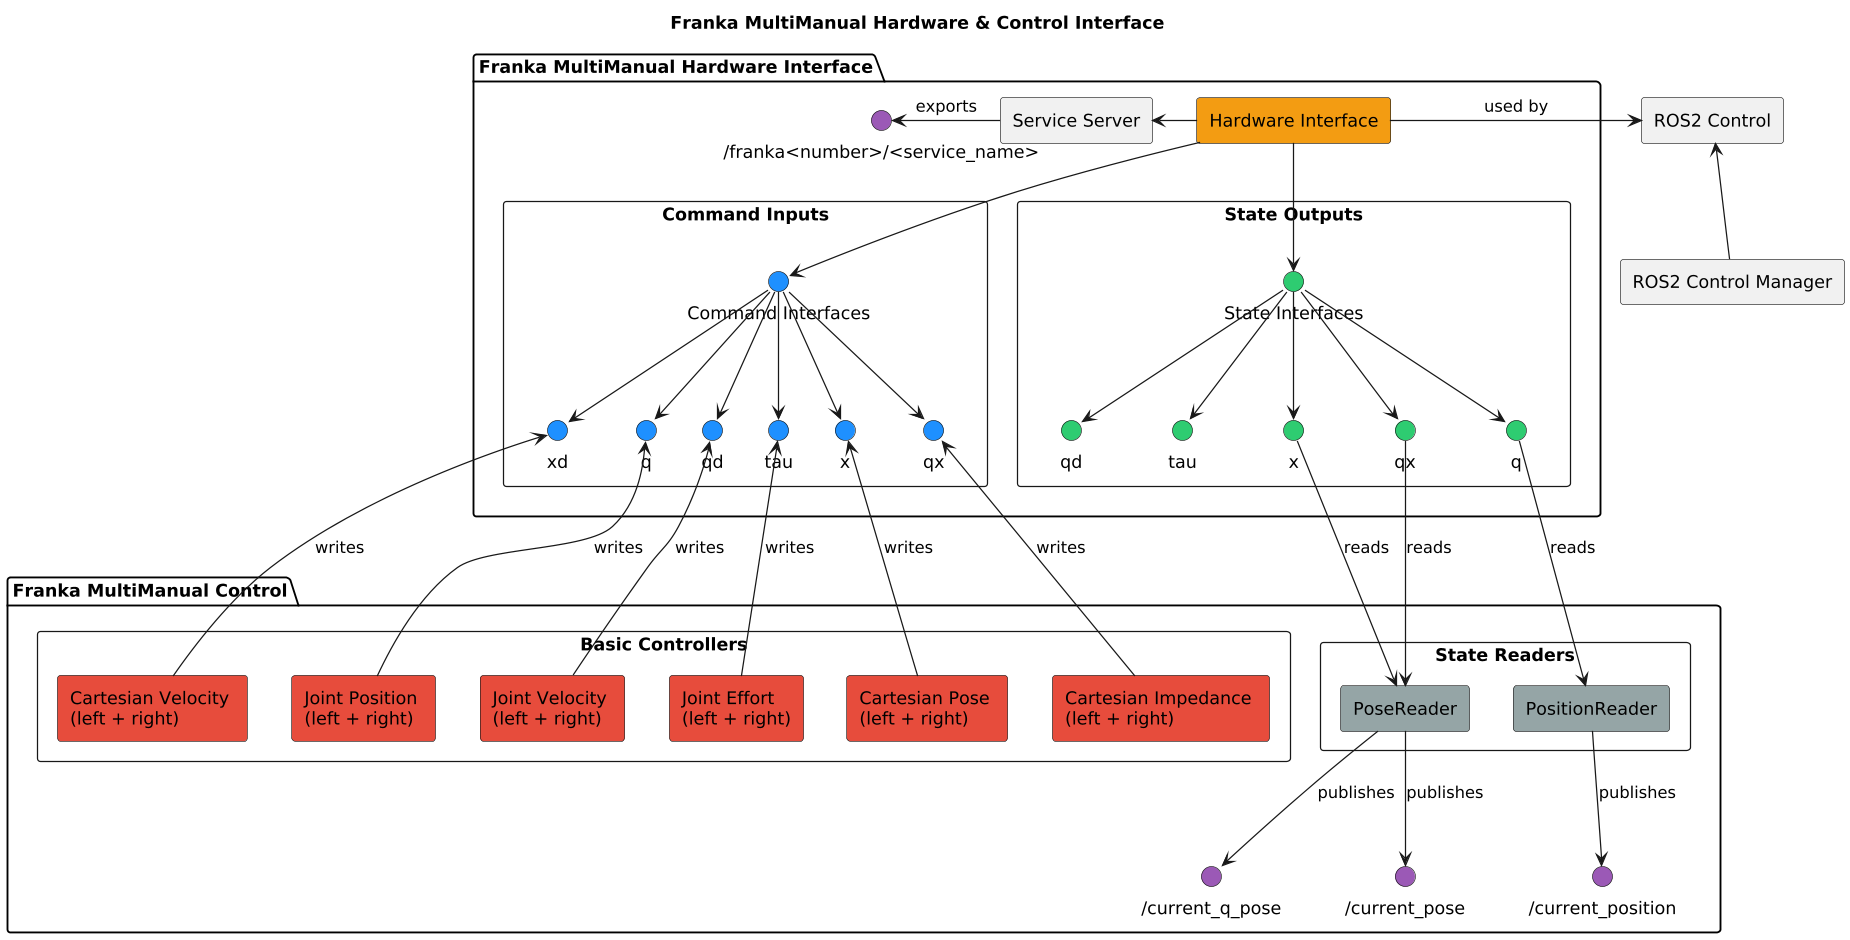
\includegraphics[width=\linewidth]{images/diagram.png}
    \caption{Communication scheme between Hardware Interface and Controller}
    \label{Figure:1}
\end{figure}

The communication between the hardware interface and the control package is summarized in Figure 1. The hardware interface package exports all the state and command interfaces that can be read and written, in addition to the service endpoints used to actively modify robot parameters. Two controllers, \texttt{PoseReader} and \texttt{PositionReader} write from particular state interfaces to make available poses and positions in their topics. The other controllers that are part of the \texttt{Basic Controllers} group, write in the command interfaces to make the robot move accordingly to the desired values.

\section{Idra Franka Launch}

These packages define the URDF used to define the robot structure and the launch file to activate two robots.

\subsection{Franka description and Bimanual URDF}

The actual URDF defined for the bimanual robot is defined inside it's own file and uses Franka description macros. It defines the shape of the table, the bases and their locations with respect to the table. The two robots are spawned with the macros defined in Franka files and attached to their base plates. 
To have a correct control of the robots, it was necessary to redefine the ROS2 control tag: this was done because spawning two franka robots makes the macros create two different ros2 control tags, creating conflicts between them. To simply remove the tag from Franka URDF files, it is possible to suppress them passing \texttt{ros2\_control = false} as argument to the robot macro.

\subsection{Launch file}
This file launches the robot, both in emulated and in real contexts. The launch file, thanks to it's numerous parameters automatically handles all the necessary operations such as the launch of Gazebo and RViz, the loading and activation of the controllers and the robot spawn. This list enumerates the parameters used in the file, explaining their role and how they should be used:
\begin{description}
    \item[load\_gripper] If set to true, loads the robot with a gripper and spawns the Gripper Action Servers.
    \item[gripper\_type] Expresses the type of the loaded gripper, franka\_hand or cobot\_pump.
    \item[use\_rviz] Set to true if RViz must be opened at startup.
    \item[use\_gazebo] Set to true if the the robot must be simulated in a virtual environment. If set, robots will also be spawned in Gazebo. Because the robots are simulated, robot IPs will be ignored.
    \item[enable\_self\_collisions]: If set to true, enables robot self-collisions.
    \item[use\_fake\_hardware]: If set to true, spawn a Generic System instead of the actual hardware interface.
    \item[use\_fake\_sensor\_commands]: If set to true, Gazebo will create mock sensor commands.
    \item[limit\_override] If set to true, skips the franka::limitRate smoothing done in the control loops.
    \item[left\_ip] IP of the robot on the left side of the table.
    \item[right\_ip] IP of the robot on the right side of the table.
    \item[controller\_path] The path of the .yaml file with the definition of the controller that will be listed in the controller manager.
\end{description}

\section{Utilities and Troubleshooting}
This section suggests some setup improvements to better control the robot and some problems encountered during the study, like DDS and discontinuities handling.

\subsection{DDS Setup}
Ros uses a DDS (Data Distribution Service) as a middleware to implement its communication protocol. It is possible to install and choose different DDS libraries to have enhanced performances during run-time. For this project Eclipse Cyclone DDS was used, utilizing the configuration of \href{https://github.com/ADVRHumanoids}{ADVR Humanoids (IIT)} group (\href{https://github.com/ADVRHumanoids/ros2_config}{here}). When calling a service, the default ROS2 DDS temporary stops the communication between nodes, while with this new configuration it does not, making communication between nodes faster and removing blocking calls of the services.

\subsection{Discontinuities}
Due to the high controller speed (1000Hz) of Franka robots, it is possible that \texttt{communication\_constraint\_violation} errors are raised, signaling that control cycles requirements are not met. 
The first thing to do is to check that you are not using Franka controls that return \texttt{ActiveControlBase} values and only use controls that are launched by the \texttt{robot.control(...)} function.
After this first check, these are the other possible causes of the error:
\begin{description}
    \item[Slow control cycle,] meaning that the implementation of the control function takes too much time to be executed. This cause is probably due to the heavy calculations done inside the cycle and it is the first to be checked.
    \item[CPU frequency scaling,] a problem caused by the CPU switching from performance to balanced/eco modes.
    \item[Networking,] all the problems related to lost packets, round-trip time and jitters. This problem could also be caused by slow switches placed in the communication path between the workstation and the robots.
\end{description}

For the last two problems,refer to the troubleshooting section of the Franka documentation.

\section{Useful links}
\begin{description}
    \item[] \href{https://frankarobotics.github.io/docs/index.html}{Franka documentation}, including librfranka, FCI, franka\_ros2 control and connection troubleshooting instructions.
    \item[] \href{https://github.com/frankarobotics}{Franka GitHub page}. Especially refer to franka\_description and franka\_ros2 repositories.
    \item[] \href{https://frankarobotics.github.io/libfranka/0.15.0/}{Libfranka class documentation}, containing the complete documentation for each class.
    \item[] \href{https://github.com/yilmazabdurrah/multi_franka_arm_ros2}{This} multi-manual implementation using Franka Panda robots.

    \item[] \href{https://docs.ros.org/en/humble/Installation/RMW-Implementations/DDS-Implementations/Working-with-Eclipse-CycloneDDS.html}{Cyclone DDS} installation guide for ROS2 and \href{https://docs.ros.org/en/humble/How-To-Guides/Working-with-multiple-RMW-implementations.html}{management of multiple instances of DDS in ROS2}.
\end{description}

\end{document}
